\documentclass{article}
\usepackage{vaibhavblayer}
\instagramp

\header{170622}{WAV}{02}[E]
\footer{4}

\usetikzlibrary{snakes}
\usepackage{annotate-equations-m}
\begin{document}

\pagecolor{white!85!orange}
\color{white!10!purple}

\def\subtitle{\small\textcolor{black!90}{considering wind}}
\def\subtitletwo{\footnotesize\textcolor{black!90}{with sign convention}}
\title{Doppler's Effect \subtitle}

\vspace*{\fill}

\begin{center}
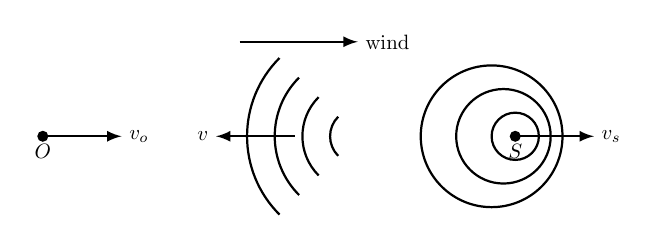
\begin{tikzpicture}[ thick, every node/.style={scale=0.75}]

\coordinate (s) at (6,0);
\coordinate (o) at (0,0);
\coordinate (w) at (4,0);

\fill (s) circle(2pt) node[below]{$S$};
\draw[-latex] (s)--+(1,0) node[right]{$v_s$};
\foreach  \r in {0.3,0.6,...,1.2}
   {
	\draw (s)++(-0.5*\r+0.15, 0) circle[radius=\r];
   };

\fill (o) circle(2pt) node[below]{$O$};
\draw[-latex] (o)--+(1,0) node[right]{$v_o$};
\draw[snake=expanding waves] (w) --+(-1.5,0);
\draw[-latex] (w)++(-0.8,0)--+(-1,0) node[left]{$v$};
\draw[-latex] (w)++(-1.5, 1.2)--+(1.5, 0) node[right]{wind};
\end{tikzpicture}
\end{center}

{\Large
\[
 f' = f_0\left( \dfrac{v - v_{\textit{wind}} + v_o}{v -v_{\textit{wind}} + v_s} \right)
\]
}
\vspace*{10 mm}

\begin{equation*}
\eqnmarkbox{fn}{f'}
\eqnmarkbox{fo}{f_0}
\eqnmarkbox{vw}{v_{\textit{wind}}}
\eqnmarkbox{v}{v}
\eqnmarkbox{vo}{v_o}
\eqnmarkbox{vs}{v_s}
\end{equation*}
\annotate[yshift=-0.2em]{below, left}{fn}{\texttt{observed frequency}}
\annotate[yshift=-1.2em]{below,left}{fo}{\texttt{source frequency}}
\annotate[yshift=-2.2em]{below,right}{v}{\texttt{velocity of sound in the medium}}
\annotate[yshift=-1.2em]{below,right}{vo}{\texttt{velocity of observer}}
\annotate[yshift=-0.2em]{below,right}{vs}{\texttt{velocity of source}}
\annotate[yshift=-2.2em]{below, left}{vw}{\texttt{velocity of wind}}
\vspace*{\fill}
\end{document}
